% ******************************* Thesis Appendix A ****************************
\chapter{The code and inputs}

\section{Building the dislocation}
\label{sec:building_disloc_code}

Given below are a set of python functions to build an array of atoms in the form described in \autoref{sec:build}. Also defined are some example inputs such as the input for the NaCl slip systems.
 Typical use would be to import this as a module to a script and use the first three functions.
 
 
\lstinputlisting{Appendix_1/build.py}

\section{Inputs}
\label{sec:pyerls_inputs}

\subsection{Elastic Tensors for cementite under different levels of hydrogen loading.}
\label{sec:elastic_tensors}

The elastic tensors for cementite loaded with varying amounts of hydrogen used for a Peierls analysis, discussed in \autoref{sec:elastic_results}, are given below. These were calculated by DFT using CASTEP \cite{Clark2005} by Miles Stopher and David Bombac, see \cite{Stopher2017} for more details. 

\begin{align*}
C_{ij}^{\text{0H}} &= \begin{pmatrix}
387.2 & 153.0 & 155.4 & 0     & 0    & 0 \\
153.0 & 342.7 & 158.0 & 0     & 0    & 0 \\
155.4 & 158.0 & 308.5 & 0     & 0    & 0 \\
0     & 0     & 0     & 133.1 & 0    & 0 \\
0     & 0     & 0     & 0     & 16.8 & 0 \\
0     & 0     & 0     & 0     & 0    & 132 \\
\end{pmatrix} \\
C_{ij}^{\text{5H}} &= \begin{pmatrix}
373.7 & 155.3 & 128.4 & -1.7 & 3.4 & 6.3 \\
155.3 & 343.6 & 173.8 & 3.3 & -7.3 & -0.8 \\
128.4 & 173.8 & 286.6 & 2.6 & -9.9 & 1.7 \\
-1.7 & 3.3 & 2.6 & 128.9 & -8 & 0.2 \\
3.4 & -7.3 & -9.9 & -8 & 32.3 & -1 \\
6.3 & -0.8 & 1.7 & 0.2 & -1 & 130.1 \\
\end{pmatrix} \\
C_{ij}^{\text{7H}} &= \begin{pmatrix}
341.3 & 134.2 & 127.6 & 0 & 0 & 4.4 \\
134.2 & 306.1 & 162.6 & 0 & 0 & 3.4 \\
127.6 & 162.6 & 288.6 & 0 & 0 & 18.9 \\
0 & 0 & 0 & 64.6 & 0.8 & 0 \\
0 & 0 & 0 & 0.8 & 27.7 & 0 \\
4.4 & 3.4 & 18.9 & 0 & 0 & 103.5 \\
\end{pmatrix} \\
C_{ij}^{\text{10H}} &= \begin{pmatrix}
331.4 & 127.2 & 130.5 & 0 & 0 & -6.8 \\
127.2 & 222.8 & 140.1 & 0 & 0 & 1.3 \\
130.5 & 140.1 & 279.5 & 0 & 0 & -0.3 \\
0 & 0 & 0 & 95.3 & 3.8 & 0 \\
0 & 0 & 0 & 3.8 & 61.4 & 0 \\
-6.8 & 1.3 & -0.3 & 0 & 0 & 44.3 \\
\end{pmatrix}
\end{align*}

\section{Analysing the results}
\label{sec:analysing_results_code}

\section{Ionic energy calculations}
\label{sec:ionic_energy_code}
%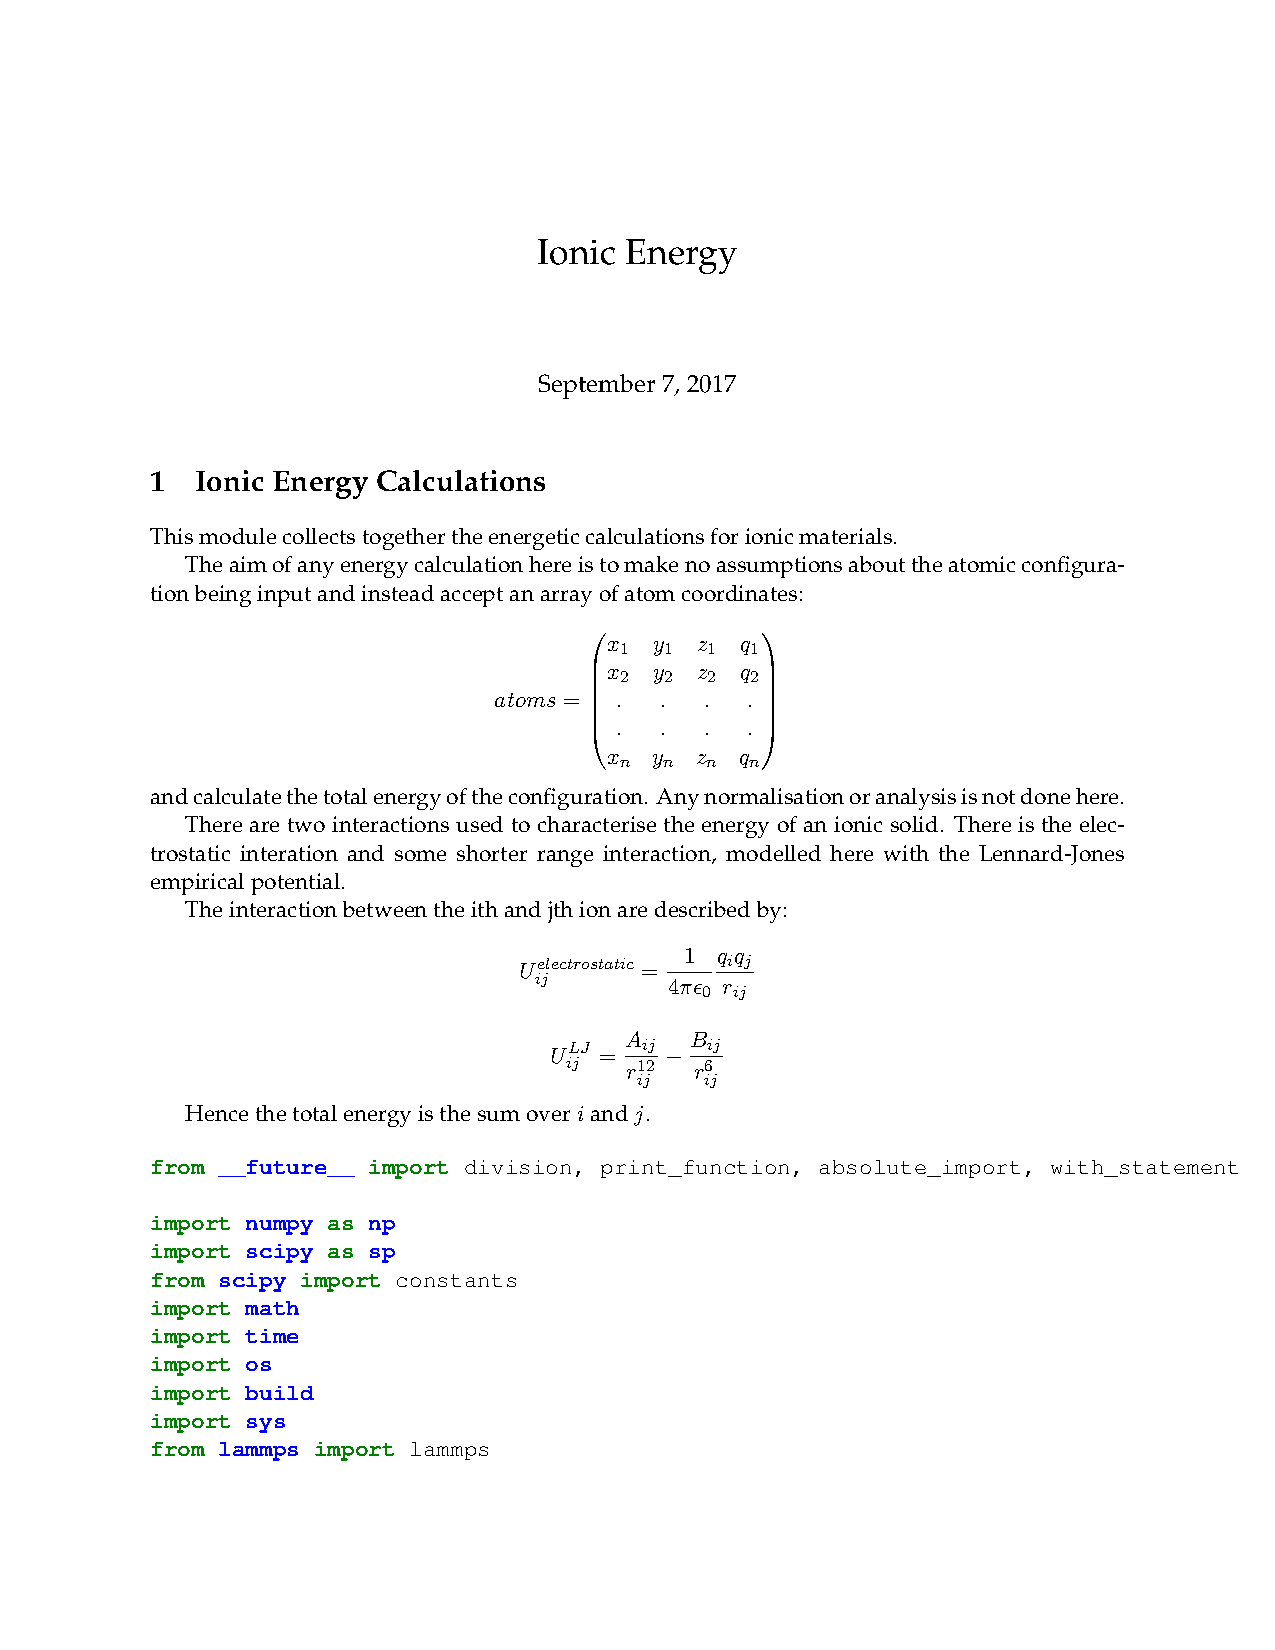
\includepdf[pages=-]{Appendix1/ionic-energy.pdf}


\section{LAMMPS inputs}
\label{sec:lammps_input}
